\documentclass[tikz]{standalone}
\usetikzlibrary{arrows,decorations.markings}
\begin{document}
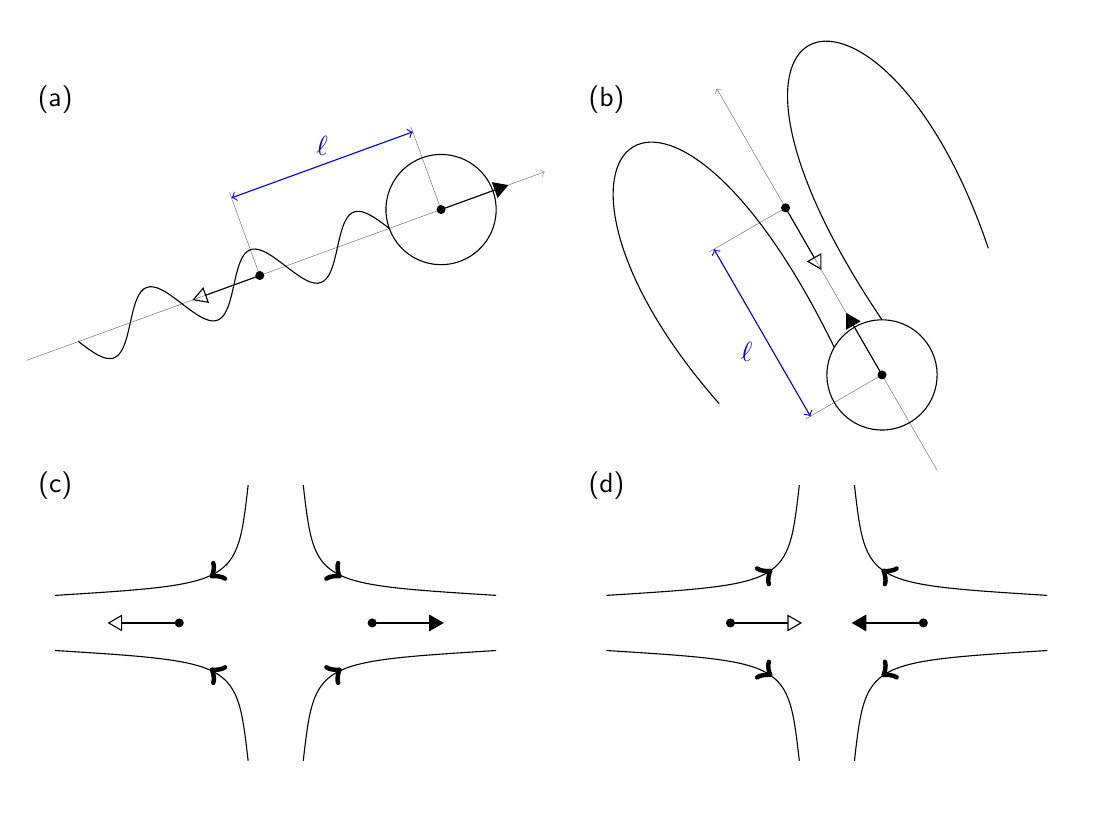
\begin{tikzpicture}[scale=.7,dot/.style={draw,fill,circle,inner sep=1pt},
  flow/.style={postaction=decorate,decoration={
      markings,mark=at position .65 with {\arrow[line width=2pt]{#1}}
    }}]
  \useasboundingbox (-7.5,-10.5) rectangle (11.5,3.3);
  \node at (-7,+2) {\textsf{(a)}};
  \node at (+3,+2) {\textsf{(b)}};
  \node at (-7,-5) {\textsf{(c)}};
  \node at (+3,-5) {\textsf{(d)}};
  \begin{scope}[rotate=20]
    \draw[help lines,->] (-8,0) -- (2,0);
    \draw[help lines] (0,0) -- (0,1.6) (-3.5,0) -- (-3.5,1.6);
    \draw (0,0) circle (1);
    \draw plot[domain=-7:-1,samples=51,smooth] (\x,{.5*sin(pi*\x r)});
    \draw[-triangle 60] (0,0) node[dot] {} -- node[below] {} (1.3,0);
    \draw[-open triangle 60] (-3.5,0) node[dot] {} -- node[below] {} ++(-1.3,0);
    \draw[blue!80!black,<->] (0,1.5) -- node[above] {$\ell$} (-3.5,1.5);
  \end{scope}
  \begin{scope}[shift={(8,-3)},rotate=120]
    \draw[help lines,->] (-2,0) -- (6,0);
    \draw[help lines] (0,0) -- (0,1.6) (3.5,0) -- (3.5,1.6);
    \draw (0,0) circle (1);
    \draw (+30:1) .. controls (0:8) and (+30:8) .. (+70:3);
    \draw (-30:1) .. controls (0:8) and (-30:8) .. (-70:3);
    \draw[-triangle 60] (0,0) node[dot] {} -- node[below] {} (1.3,0);
    \draw[-open triangle 60] (3.5,0) node[dot] {} -- node[below] {} ++(-1.3,0);
    \draw[blue!80!black,<->] (0,1.5) -- node[below left] {$\ell$} (3.5,1.5);
  \end{scope}
  \begin{scope}[shift={(-3,-7.5)}]
    \draw[-triangle 60] (1.75,0) node[dot] {} -- ++(1.3,0);
    \draw[-open triangle 60] (-1.75,0) node[dot] {} -- ++(-1.3,0);
    \draw[flow=<] (-4,+.5) .. controls (135:1) .. (-.5,+2.5);
    \draw[flow=<] (-4,-.5) .. controls (225:1) .. (-.5,-2.5);
    \draw[flow=<] (+4,+.5) .. controls ( 45:1) .. (+.5,+2.5);
    \draw[flow=<] (+4,-.5) .. controls (315:1) .. (+.5,-2.5);
  \end{scope}
  \begin{scope}[shift={(7,-7.5)}]
    \draw[-triangle 60] (1.75,0) node[dot] {} -- ++(-1.3,0);
    \draw[-open triangle 60] (-1.75,0) node[dot] {} -- ++(1.3,0);
    \draw[flow=>] (-4,+.5) .. controls (135:1) .. (-.5,+2.5);
    \draw[flow=>] (-4,-.5) .. controls (225:1) .. (-.5,-2.5);
    \draw[flow=>] (+4,+.5) .. controls ( 45:1) .. (+.5,+2.5);
    \draw[flow=>] (+4,-.5) .. controls (315:1) .. (+.5,-2.5);
  \end{scope}
\end{tikzpicture}
\end{document}
